\documentclass[oneside]{article}
\usepackage[utf8]{inputenc}

\title{Enhancement of Matrix Multiplication using Parallelization and Evolutionary Strategies \\ \vspace{2 mm} {\Large Preliminary Progress Report}}
\author{Jonathan Gillett}
\date{March 2015}

\usepackage{natbib}
\usepackage{graphicx}
\usepackage{url}
\usepackage{setspace}
\usepackage[ruled,vlined]{algorithm2e}

\begin{document}

\maketitle



\section{Abstract}

\doublespacing
Matrix multiplication is among one of the most widely used and extensively studied operations in computing\cite{raz2002complexity}. The complexity of the naive implementation is $O(N^{3})$\cite{raz2002complexity}, with the theoretical lower bound of this computation shown to be $\Omega(N^{2})$\cite{raz2002complexity}. Despite the difference between the upper and lower bounds, the naive implementation remains the most widely used due to the optimization of cache hits\cite{note2002reducing}; much research has been invested in finding more optimal methods of performing this operation.

Advances in optimizing matrix multiplication, such as the Strassen and Coppersmith–Winograd algorithms\cite{huss1996implementation, coppersmith1987matrix} have focused on limiting the number of expensive multiplication operations performed in order to reduce the computational complexity. Despite the theoretical lower complexity of these algorithms, the performance benefits are often negated by the practical limitations of the implementations for real-world datasets and extremely large constants\cite{robinson2005toward}.

Rather than focusing on theoretical optimizations, recent trends have focused on using approximate methods and recent advances in parallelism based on MapReduce, which is provided by the Hadoop framework\footnote{Hadoop is a distributed file system and parallel computation framework\cite{shvachko2010hadoop} often used for performing MapReduce operations based on specifications published by Google researchers\cite{dean2008mapreduce}}. Large technology companies such as Twitter and Facebook have realized the performance benefits of approximate parallel matrix multiplication operations to perform data analysis and machine learning to maximize ad revenue. Twitter, in particular created an approximate matrix multiplication operation known as DIMSUM, to perform parallel approximate matrix multiplication using MapReduce on matrices hundreds of terabytes in size\cite{zadeh2013dimension}.

Given the recent trend towards approximate parallel computation for matrix multiplication, the emphasis of the research will be to focus on implementing an approximate solution for matrix multiplication. Time permitting, the resaerch will optimize the process further using parallelization and evolutionary strategies to optimize parameters.

For the preliminary results we have implemented a test framework in order to consistently test and validate the different implementations. Currently there are three benchmark implementations that have been created: a naive solution demonstrating the poor performance of iteration in Python; a baseline solution, which uses the \emph{np.dot} function provided by the NumPy library; and finally, a simple parallel implementation using MPI, where the rows are divided amongst N processors.

The desired outcome for the final report is that additional parallel implementations will be created, and an approximate implementation based directly on the work of Drineas and Kannan\cite{drineas2001fast}. The challenge in implementing the approximate solution is to comprehend the theorems and lemmas and to understand their methodology, such that it can be translated into Python and the results reproduced. Lastly, the final goal for the research, time permitting, would be to incorporate parallelism and evolutionary strategies into the approximate implementation.



\section{Introduction}

Matrix multiplication is fundamental to computing, and is an operation widely studied and used in numerical analysis with many real-world applications. The naive implementation has a complexity of $O(N^{3})$\cite{raz2002complexity} with a theoretical lower bound shown to be $\Omega(N^{2})$\cite{raz2002complexity}. For very large matrices this difference can have a major impact in the amount of time required for computations.

However, even though the complexity of the naive implementation is significantly higher than the lower bound, it is still widely used due to highly optimized implementations written in Fortran, that make use of optimal cache hits\cite{note2002reducing}. The performance of the naive algorithm and other linear algebraic operations is so critical that software such as LAPACK (Linear Algebra PACKage)\cite{lapackweb} and ATLAS (Automatically Tuned Linear Algebra Software)\cite{whaley2001automated} have been created to provide optimal implementations of these operations. LAPACK provides many common operations for linear algebra such as matrix multiplication, and has been invaluable to the progress of both academia and industry. Furthermore, LAPACK is also fundamental to the success of MATLAB\cite{matlab2000}, which is one of the most widely used software applications in science and engineering.

In addition to optimizing the implementations of the naive method of matrix multiplication, there have been many recent advances in optimizing the theoretical complexity of matrix multiplication starting with the Strassen and Coppersmith–Winograd algorithms\cite{huss1996implementation, coppersmith1987matrix}. These algorithms have focused on limiting the number of expensive multiplication operations performed in order to reduce the computational complexity. In Strassen's algorithm the number of multiplication operations required is reduced, giving a slightly lower complexity of $O(N^{2.8074})$\cite{huss1996implementation}. In the case of the Coppersmith–Winograd algorithm, which is similar to Strassen's, the complexity is $O(N^{2.374})$\cite{stothers2010complexity}. Nevertheless, despite the theoretical lower complexity of these algorithms, their use of recursion negatively impacts cache access, and the theoretical performance benefits are negated by the more optimal naive implementations, which make use of optimal cache hits\cite{note2002reducing}. In particular, the large constants of the Coppersmith-Winograd algorithm make it only feasible for extremely large matrices, beyond the storage and memory capabilities of present day hardware\cite{robinson2005toward}.

As a result of the practical limitations of the theoretically optimal matrix multiplication algorithms, research and industry have been swift to focus on optimizations of matrix multiplication that sacrifice exact for approximate solutions and make use of highly parallel algorithms. The work by Drineas and Kannan in their seminal paper, \emph{Fast Monte-Carlo Algorithms for Approximate Matrix Multiplication}\cite{drineas2001fast}, and their subsequent three part publication in SIAM\cite{drineas2006fastI, drineas2006fastII, drineas2006fastIII}, laid the groundwork for much of the modern-day approaches to performing approximate linear algebraic operations. Building on the body of research conducted with Drineas and Kannan, Mahoney continued to pursue further applications of approximate stochastic algorithms to algebraic operations. In 2011 Mahoney published a detailed review paper on the subject, \emph{Randomized Algorithms for Matrices and Data}\cite{mahoney2011randomized}, which became highly influential to industry with it's numerous practical applications to machine learning.

The significance of this research caught the attention of Twitter and Facebook, which are data driven organizations that rely on linear algebraic operations for machine learning and data analysis. Twitter created an approximate matrix multiplication operation known as DIMSUM. DIMSUM was used to perform parallel approximate matrix multiplication with MapReduce on matrices hundreds of terabytes in size, and resulted in significant performance improvements\cite{zadeh2013dimension}.


\begin{figure}[ht!]
\centering
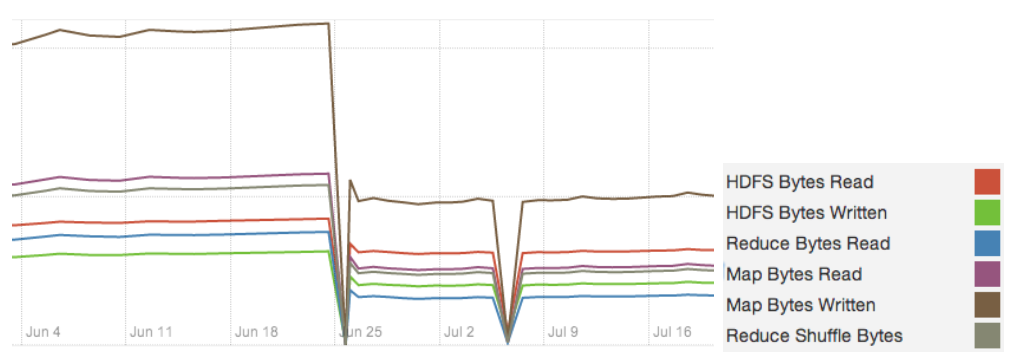
\includegraphics[width=\textwidth]{figures/twitter-dimsum}
\caption{DIMSUM, used in production at Twitter since June 2014, has resulted in an observed 40\% performance improvement\cite{zadeh2013dimension}}
\label{fig:transaction}
\end{figure}


Given the importance of optimizing matrix multiplication and the recent emphasis on utilizing approximate stochastic methods and parallelism. Studying these topics is an interesting problem that is relevant to the course given the emphasis on numerical precision and parallelism in High Performance Computing (HPC). Therefore, the purpose of this project will be to focus on the common serial implementations of matrix multiplication and to study the performance benefits of parallel and approximate implementations. Matrix multiplication is a very well defined problem, where the results can be easily verified and benchmarked using the tools and techniques demonstrated in class with Python, Numpy, and MPI\cite{van2011numpy}.

The greatest challenge will be implementing the approximate solutions, which involves reading through papers by Drineas, Kannan, and Mahoney in order to comprehend the theorems and lemmas and to understand their methodology and into Python. Following this, the next challenge will be to implement parallel algorithms for matrix multiplication, for example Cannon's algorithm. Considering that Python is inherently a single process/single threaded language due to the Global Interpreter Lock (GIL)\cite{beazley2010understanding}, parallelism will be implemented using MPI, following the techniques and examples demonstrated in lectures.




\section{Problem Formulation}

Matrix multiplication is a linear algebraic operation that is a fundamental step in many operations in computing. Similarly to the importance of multiplication to arithmetic, matrix multiplication is critical to performing operations on systems of equations and other models for computation. The naive method for matrix multiplication, as shown in algorithm \ref{alg:naive}, involves three nested iterations and intuitively has a computational complexity of $O(N^{3})$.

\begin{algorithm}[!ht]
  \SetKwProg{Fn}{}{}{end}
  \SetKwFunction{Naive}{Naive}
  \SetKwArray{Forwards}{forwards}
  \SetKwFunction{ZeroMatrix}{zeroMatrix}
  \SetAlgoNoLine
  \DontPrintSemicolon
  
  \Fn{\Naive{$A, B$}}{
  \tcp{C is a zero matrix with dimensions from A, B}
  $C \leftarrow $ \ZeroMatrix($A_{rows}, B_{cols}$)
  \BlankLine
  
  \For{$i \leftarrow 1$ \KwTo $A_{rows}$}
  {
    \For{$j \leftarrow 1$ \KwTo $B_{cols}$}
    {
      \For{$k \leftarrow 1$ \KwTo $A_{cols}$}
      {
        $C_{i, j} \leftarrow C_{i, j} + A_{i, k} * B_{k, j}$
      }
    }
  }
  \BlankLine
  \KwRet($C$)
}
\caption{Naive Matrix Multiplication}
\label{alg:naive}
\end{algorithm}


The problem at hand involves studying the optimizations of the naive matrix multiplication and utilizing approximate and parallel solutions based on existing literature, and research to improve it. Furthermore, in order to consistently measure the performance improvements of the approximate and parallel implementations, a test framework must be created. The test framework will be used to execute each of the implementations against a variety of test matrices and to perform numerous trials in order to record accurate statistical results. The results of each implementation will then be compared to the performance results of the naive implementation provided by the \emph{np.dot} function, which is part of the NumPy library.




\subsection{Solution Methodology}

In order to complete this project the solution methodology will consist of selecting suitable matrices of different sizes so that the performance benchmarks are consistent and accurate. Following this, a framework for testing the implementations will be produced to automate testing each implementation against a set of matrices determined for the experiments. Lastly, each of the proposed approaches will be evaluated and each implementation will be benchmarked and compared to the baseline result of the serial naive implementation.

The following is the revised solution methodology, based on the initial project proposal.

\begin{enumerate}
\item For the purpose of benchmarking, a set of suitable matrices will be defined, in particular large matrices representing graphs and stochastic models will be used based on their numerous applications\cite{yegnanarayanan2013application}.

\item The results for the approximate algorithms will be compared to the exact results of the \emph{np.dot} operation using the norm of the error matrix, which results from the subtraction of the approximate matrix, $P$, from the exact result, $P - A \cdot B$\cite{drineas2001fast}. Furthermore, for the test matrices representing stochastic models, the steady-state eigenvalues will also be compared and recorded during the benchmarking.

\item A Python test framework will be created that will execute all of the tests and record the execution times and the result of multiplication calculations. This will be used to automate the benchmarking process and consistently and accurately benchmark the parallel and approximate implementations and evaluate the results.

\item The serial baseline benchmark will be implemented using the \emph{np.dot} operation and tested using the framework as a base reference to compare against each of the approximate and parallel implementations.

\item Parallel algorithms such as Cannon's algorithm\cite{lee1997generalized}, will be implemented using MPI and Numpy and tested using the framework. The results will be compared to the performance of the baseline implementation.

\item Approximate algorithms will be implemented directly based on the paper, \emph{Fast Monte-Carlo Algorithms for Approximate Matrix Multiplication}\cite{drineas2001fast}, by Drineas and Kannan.

\item Time permitting, evolutionary strategies such as genetic algorithms and differential evolution, which are often used in optimization\cite{de1989using}, will be used to optimize parameters for the approximate algorithms.

\item All implementations will be compared against each other and the reference baseline using the framework and the performance results and the margin of error, for approximate implementations, will be recorded.
\end{enumerate}




\section{Preliminary Results}

The preliminary results so far have been the creation of several implementations that can be used to compare the performance of matrix multiplication, including the baseline implementation, a slower naive implementation demonstrating the poor performance of iteration in Python, and lastly a simple parallel implementation using MPI.

In addition to creating several implementations, a test framework has also been created to automate the process of benchmarking implementations and comparing the results. The test framework parses a test plan document, which is written using YAML, that describes each of the benchmark codes, the tests, the matrices used for the tests, and the order in which tests are executed. The following snippet shows the versatility of the test plan YAML document that is parsed by the test framework.


\singlespacing
\begin{verbatim}
benchmarks:
    - name: simple_parallel
      description: Simple parallel implementation using MPI
      file: simple_parallel.py
      exec: mpiexec
      args: ['-np', '4', 'python2']
tests:
    - name: assorted_float
      description: Tests with uniform floats of [0, 1).
      dimensions: [25, 50, 75]
      type: float
testplan:
    - test: assorted_float
      trials: 10
\end{verbatim}


\doublespacing
The creation of the test framework greatly simplifies the process of executing the benchmarks and validating the performance results by automating the entire process. All that is required for the test framework are the benchmarks and a test plan. The test plan outlines the test cases to execute; the test matrices to generate; the codes to execute; and the order in which tests are to be executed. The test framework then parses this test plan and executes it displaying the progress of each test as shown in figure \ref{fig:progress}. After the test plan is completed summary statistics are displayed. As shown in figure \ref{fig:summary} a table displays the total average execution time for each of the benchmarks and their respective test results. In this example the \emph{simple\_parallel} implementation is marginally slower than the baseline.

\begin{figure}[ht!]
\centering
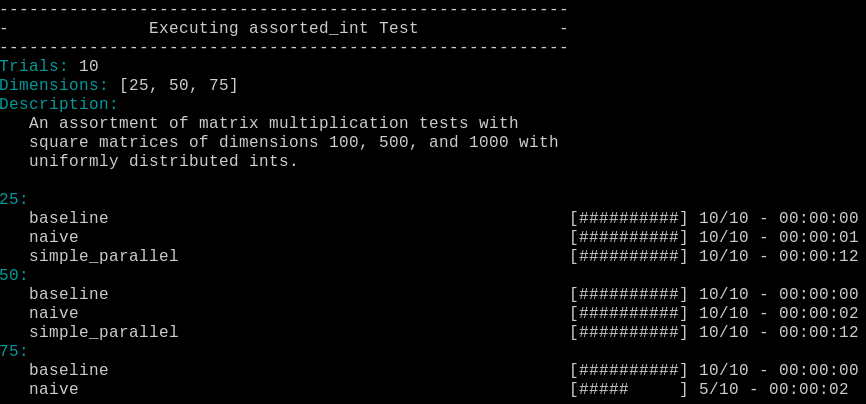
\includegraphics[width=\textwidth]{figures/framework-progress}
\caption{Test framework displaying test progress}
\label{fig:progress}
\end{figure}

\begin{figure}[ht!]
\centering
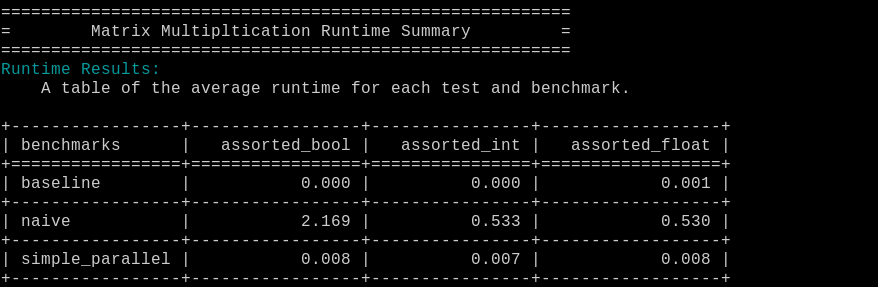
\includegraphics[width=\textwidth]{figures/framework-summary}
\caption{Test framework displaying summary statistics}
\label{fig:summary}
\end{figure}



\subsection{Expected Outcomes}

The following is the list of expected outcomes, which as been refined from the initial project proposal based on the preliminary results.

\begin{enumerate}
\item Support for generating large adjacency matrices representing graphs and stochastic matrices representing datasets that are similar to real world applications.

\item Refinement of the test framework to support evaluating approximate matrix multiplication implementations and evaluating the resultant matrix using the norm of the error matrix. As well, in the case of stochastic matrices by comparing the steady-state eigenvalues.

\item More parallel implementations, in particular an implementation based on Cannon's algorithm, which is one of the most widely used methods for parallel matrix multiplication.

\item Approximate implementations directly based on the paper, \emph{Fast Monte-Carlo Algorithms for Approximate Matrix Multiplication}\cite{drineas2001fast}, by Drineas and Kannan.

\item A final report discussing the approximate and parallel implementations, their practical applications to large adjacency and stochastic matrices, in addition to a thorough analysis of the performance results in comparison to the baseline implementation.

\end{enumerate}


\bibliographystyle{plain}
\singlespacing
\bibliography{references}
\end{document}
